
\subsection{Reaction Wheel Configuration}

angular acceleration demand \cite{reactionWheelConfigThesis} 

gps orientation, Earth station

Tetrahedron configuration can output twice as much force along an axis as one wheel can produce along its own axis.

\subsubsection{Transformation Between Body \& Reaction Wheel Space}

The main attitude controller sends torque demands to the actuators. The torque demand distributed to the reaction wheels have to be converted to torques parallel to reaction wheel axes, in order for the motor controllers to function. Transformation from reaction wheel space to body frame is quite intuitive. Knowing the orientation of each motor axis and the corresponding motor torque 
, the torque in body frame can be derived according to equation \ref{eq:motorTrans1} - \ref{transmatrix}. The matrix for tetrahedron configuration is given by \cite{reactionWheelConfigThesis}.

\begin{equation}
\label{eq:motorTrans1}
\vec{N_{rw}} = \underline{A}_{DC} \vec{N_{DC}} = \begin{bmatrix}
\vec{Axis^{DC}_{1}}       & \vec{Axis^{DC}_{2}}   & \vec{Axis^{DC}_{3}}   & \vec{Axis^{DC}_{4}} 
\end{bmatrix} \vec{N_{DC}}
\end{equation}

\begin{equation}
\underline{A}_{DC} \vec{N_{DC}}  = 
\begin{bmatrix}
\cos(19.47)       & -\cos(19.47) \cos(60)  &  -\cos(19.47) \cos(60)  & 0 \\
0       & \cos(19.47) \cos(30)  &  -\cos(19.47) \cos(30)  & 0 \\
-\sin(19.47)       & -\sin(19.47)   &  -\sin(19.47)   & 1
\end{bmatrix} \vec{N_{DC}}
\label{transmatrix}
\end{equation}

where $\vec{N_{rw}}$ is the reaction wheel torque in body frame, $\vec{N_{DC}}$ is the vector containing the reaction wheel DC motor torques parallel to their axes, $\vec{Axis^{DC}_{i}}$ are the reaction wheel motor orientation in body frame, $\underline{A}_{DC}$ is the transformation matrix between axis oriented reaction wheel torque and torques in 3 dimensional body frame.


\nomenclature[S]{$\vec{N_{rw}}$}{Reaction wheel torque in body frame }
\nomenclature[S]{$\vec{N_{DC}}$}{$4\times1$ vector containing the reaction wheel motor motor torques parallel to their axes }
\nomenclature[S]{$\underline{A}_{DC}$}{Transformation matrix between axis oriented reaction wheel torque and torques in 3 dimensional body frame }

Since $\underline{A}_{DC} $ is a $ 4 \times 3 $ matrix, a pseudo inverse has to be used when reordering the equation, as presented in equation \ref{eq:motorTrans}. 

\begin{equation}
\label{eq:motorTrans}
\vec{N_{DC}} =  \underline{A}_{DC} ^\dagger \vec{N_{rw}}   =  \underline{A}_{DC}^T  (\underline{A}_{DC} \underline{A}_{DC} ^T)^{-1} \vec{N_{DC}}
\end{equation}


%\begin{equation}
%h_{rot} = A\left[ h_1, h_2, h_3, h_4 \right]^T
%\end{equation}

In case there's a demand to adjust the torque distribution between the wheels, an extra vector can be included, as shown in equation \ref{eq:TorqueDistrib}
\cite[equation 18.41-42]{SADC}. If k is set to 0, the norm of wheel torques are minimized.

\begin{equation}
\label{eq:TorqueDistrib}
 \vec{N_{DC}} = \underline{A}^\dagger_{DC} \vec{N_{rw}}  + k\left[1,-1,-1,1\right]^T
\end{equation}


\subsubsection{Reconfiguration}

Fault isolation for the redundant reaction wheel configuration can be done by detecting which is the reaction wheel where the fault occurred and shutting it off and redistributing the torques to the rest of the reaction wheels. This reconfiguration can be represented by swapping the corresponding faulty columns to zero vectors. For example, if a fault occurs in the 3rd reaction wheel, the transformation matrix becomes $\underline{A}_{DC,f3}$, as presented in equation \ref{eq:ReactFault}.

\begin{equation}
\label{eq:ReactFault}
\underline{A}_{DC,f3} = \begin{bmatrix}
\vec{Axis^{DC}_{1}}       & \vec{Axis^{DC}_{2}}   & \vec{0}   & \vec{Axis^{DC}_{4}} 
\end{bmatrix} 
\end{equation}

\begin{figure}[h!]
	\centering 
	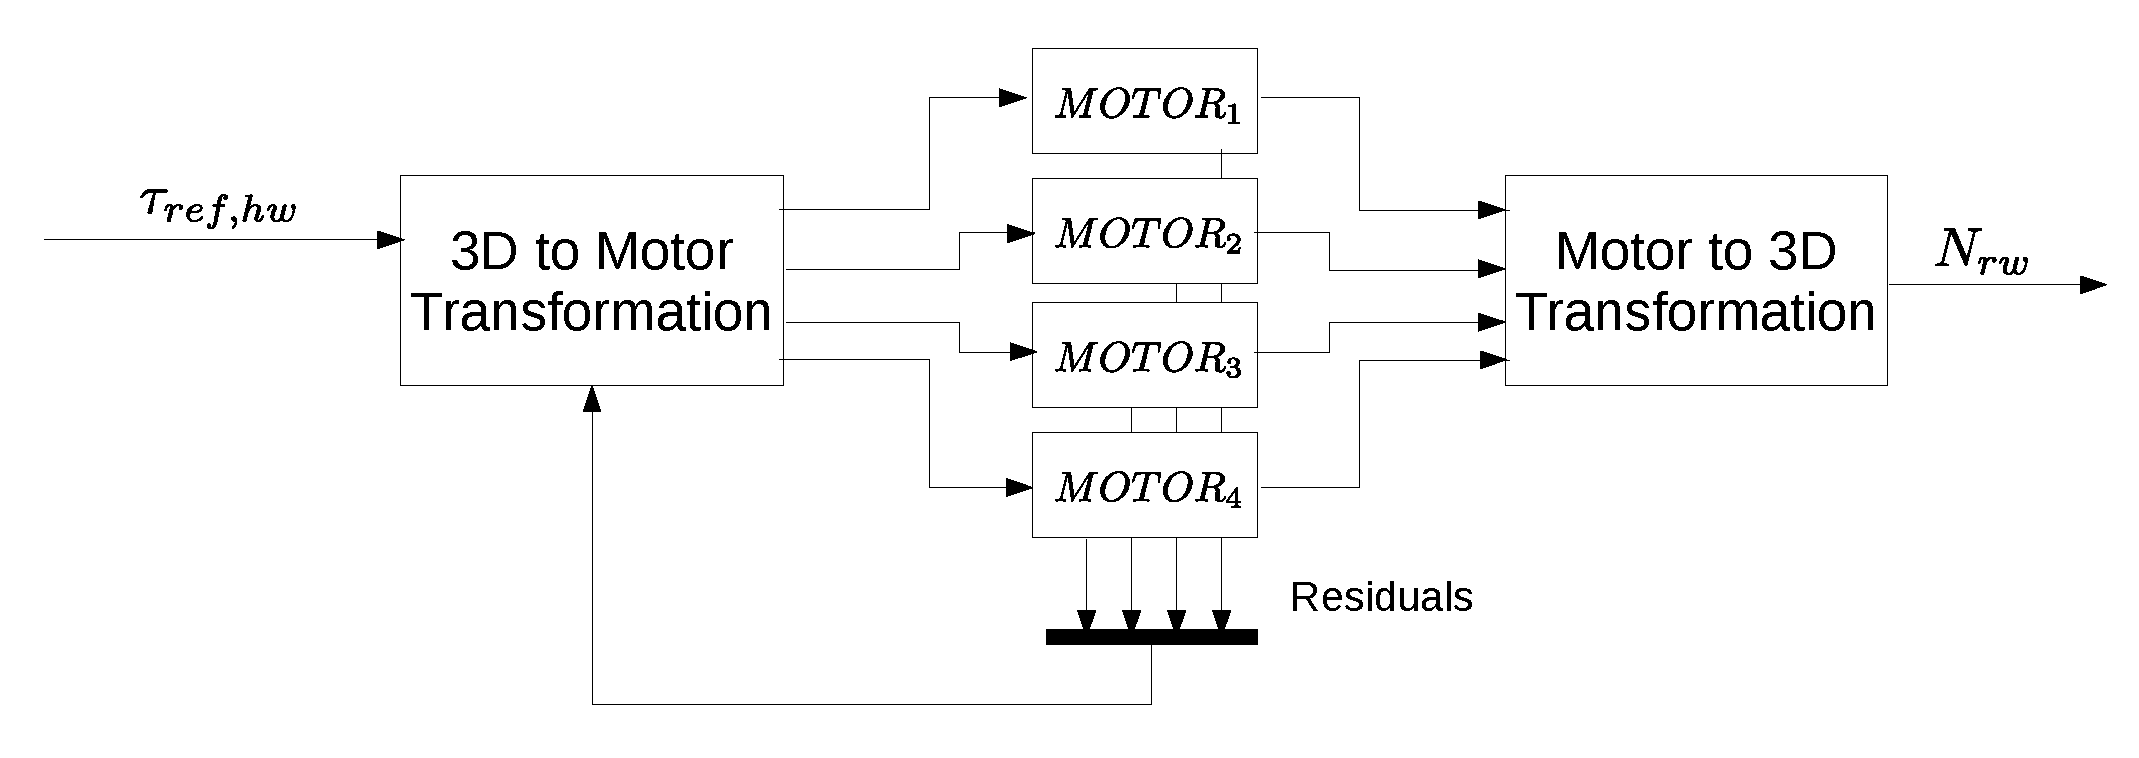
\includegraphics[width=170mm]{figures/reconfigure.pdf}	
	\caption{Reconfiguration Control Scheme for Reaction Wheels}
	\label{label{fig:reconfig}}
\end{figure}

\nomenclature[S]{$\underline{A}_{DC,fi}$}{Transformation matrix between axis oriented reaction wheel torque and torques in 3 dimensional body frame in case of faulty $i$th reaction wheel}

The pseudo inverse is calculated in the same manner as presented in equation \ref{eq:motorTrans}, as shown in equation \ref{eq:motorTransFault}. 

\begin{equation}
\label{eq:motorTransFault}
\underline{A}_{DC,f3}^\dagger   = \underline{A}_{DC,f3}^T  (\underline{A}_{DC,f3} \underline{A}_{DC,f3}^T)^{-1}
\end{equation}